O acionamento de um HSM pode ser realizado de diferentes formas para uma mesma configuração construtiva, cada forma proporciona vantagens diferentes. As principais característica que norteiam a forma de acionamento  é o número de  fases e o número de bobinas na máquina.

\subsection{Motores de Passo Unipolar e Bipolar}

Geralmente motores de passo possuem duas fases, devido principalmente a padronização dos dispositivos drives necessários para o acionamento. Logo normalmente se tem acesso apenas aos 2 terminais de cada fase. Outro ponto importante é que existem dois tipos de acionamento de polos; o acionamento unipolar e o bipolar.  

Nos motores de passo unipolar há dois enrolamentos por fase, que possuem um contato em comum, conhecido como \emph{center-tape}. Tal contato em comum pode ser usado para se colocar outras bobinas em paralelo, aumentando o numero de bobinas ativadas por passo. Porém seu principal função é servir de ponto de alimentação do motor, de modo que para controlar a corrente pelas espiras se faz necessário penas aterrar um ou os dois terminas. A figura \ref{fig:MotorDePassoUnipolar} apresenta o diagrama de um motor de passo unipolar. 

\begin{figure}[H]
	\centering
	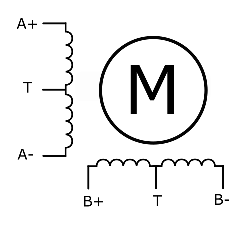
\includegraphics[width = 0.3 \columnwidth]{images/MotorDePassoUnipolar.eps}
	\caption{Motor de Passo Unipolar}
	\label{fig:MotorDePassoUnipolar}
\end{figure} 

Em relação aos terminas \emph{center-tape}, ou T como mostrado na figura \ref{fig:MotorDePassoUnipolar}, existem algumas variações de ligação onde se interliga os terminas T de modo a ficar disponível apenas 5 terminais na máquina, ou ainda onde se usa inúmeras fases todas com os terminais T curto-circuitados.   

Os motores bipolares possuem apenas uma bobina por fase, de modo que para controlar a corrente pelas espiras se faz necessário o uso de circuitos mais complexos que possam inverter a alimentação das bobinas. A grande vantagem deste tipo de motor é o maior torque em relação ao motor unipolar. A figura \ref{fig:MotorDePassoBipolar} apresenta o diagrama de um motor de passo bipolar.

\begin{figure}[H]
	\centering
	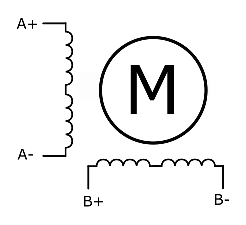
\includegraphics[width = 0.3\columnwidth]{images/MotorDePassoBipolar.eps}
	\caption{Motor de Passo Bipolar}
	\label{fig:MotorDePassoBipolar}
\end{figure}


\subsection{Modos de Acionamento} 